

\titleformat*{\subsection}{\normalsize\itshape}
\titleformat*{\section}{\normalsize\itshape}
\setcounter{section}{3}"
\section{Experiments and Discussion}
In this section, we demonstrate our experiments over three popular supervised face image datasets: \textit{the Extended Yale Face Database B} [18], \textit{AT}\&\textit{T} [19], and \textit{CelebFaces Attributes Dataset (CelebA)} [20]. To evaluate our method performance, we also conduct experiments with different generator and re-constructor structures, different types of classifications (binary and multi-class classification), different numbers of reduced dimensions. The effectiveness of the method is then evaluated in terms of utility and privacy.   
\subsection{Experiment Setup}
\textit{The Extended Yale Face Database B} (YaleB) contains 2,470 grayscale images of 38 human subjects under different illumination conditions and their identity label. In this dataset, the image size is 168$\times$192 pixels. The AT\&T dataset has 400 face images of 40 subjects. For convenience, we resize each image of these two dataset to 64$\times$64 pixels. CelebA is a color facial image dataset containing 202,599 images of 10,177 subjects. 1,709 images of the first 80 subjects are used for our experiment. Each image is resized to 64$\times$64$\times$3 pixels. All pixel values are scaled to the range of [0,1]. We randomly select 10\% of each subject's images for validation and 15\% for testing dataset. 

The generator and re-constructor in Figure \ref{fig:eGAN} are implemented by three different structures. Specifically, we follow the architecture of recent powerful models VGG19, VGG16 [33] and a basic convolutional network (CNN). We modify the models to adapt to our data size (64$\times$64). Discriminator and Classifier are built on fully connected neural network and convolutional network respectively. Leaky ReLU is used for activation function in hidden layers. We use linear activation function for generator's output layers and softmax activation functions for other components' output layers. Each component is trained in 5 local iterations ($n_r, n_g, n_d, n_c$), and the entire system is trained in 500 global iterations ($n$). The target distribution is drawn from Gaussian distribution (with the covariance value of 0.5 and the mean is the average of the training data). Table \ref{table:implementation} provides detail information of neural networks' structures and other implementation information. 

\setcounter{table}{0}
\begin{table}[H]
	\centering
	%trim  left, bottom, right and top 
	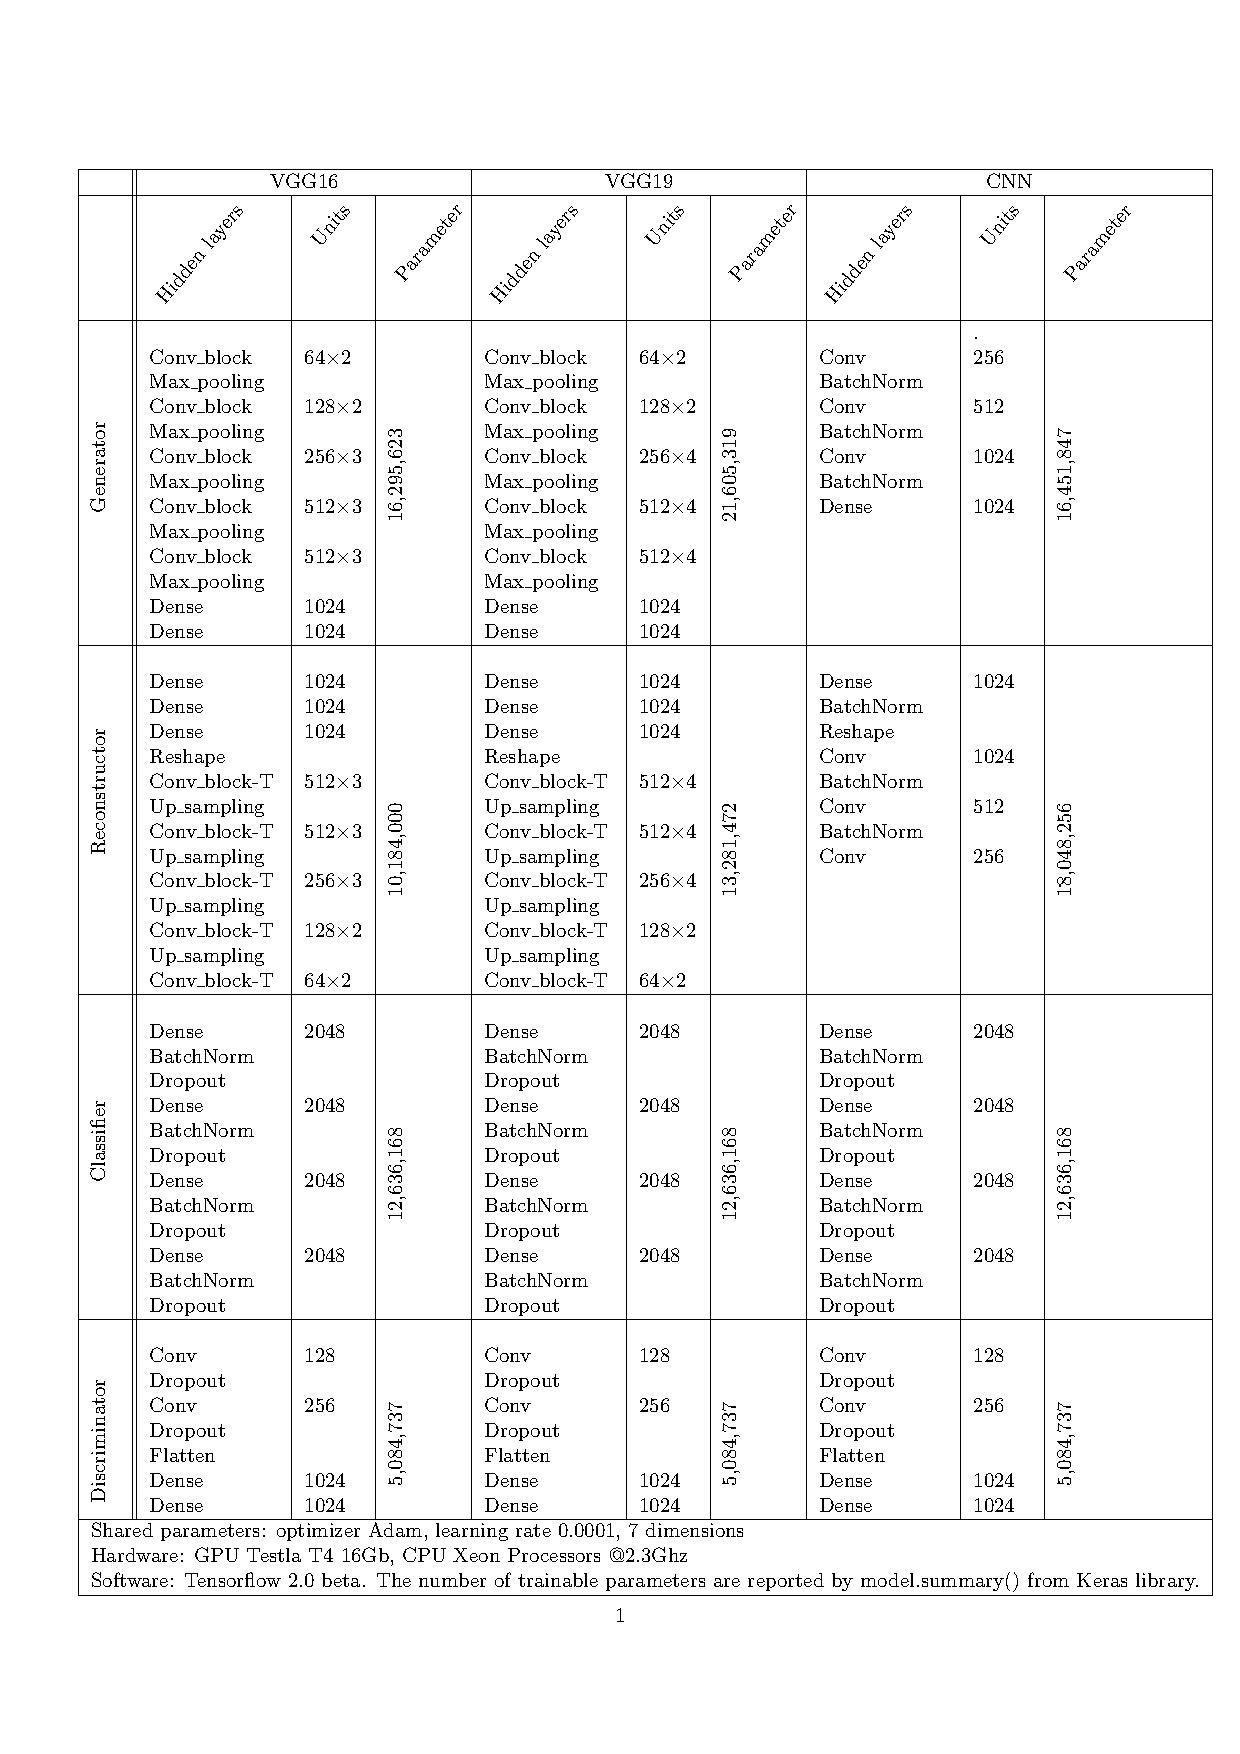
\includegraphics[width=0.7\linewidth, trim=1cm 2.5cm 0.1cm 2.5cm, clip=true]{tables/implement_table}
	\caption{Implementation information}
	\label{table:implementation}
\end{table}

To evaluate the reliability, we test our framework with different levels of authentication corresponding to binary classification (single-level) and multi-class classification (multi-level). For the single-level authentication system, we consider half of the subjects in the dataset are valid to access company's resources while the rest are invalid. We randomly divide the dataset into two groups of subjects and labels their images to (1) or (0) depending on their access permission. For the cases of multi-level authentication system, we divide the subjects into four groups and eight groups. Therefore, the authentication server becomes four-class and eight-class classifier respectively. 
\subsection{Utility}
We use accuracy metric to evaluate the utility of dimension-reduced data. The testing dataset is tested with the classifier extracted from our framework. Different structures of Generator and re-constructor are applied including VGG19, VGG16, basic CNN on different privilege levels which correspond to multi-class classification. Figure \ref{fig:acc} illustrates the accuracies for different dimensions from three to seven over the three facial datasets. Overall, the accuracies improve when the number of dimension increases. The accuracies on the two gray image datasets (AT\&T and Yale\_B) reaches 90\% and higher when using VGG with only seven dimensions. This accuracy figure for Celeba is smaller, but it still reaches 80\%. In general, VGG19 structure performs better than using VGG16 and basic CNN in terms of utility due to the complexity (table \ref{table:implementation}) and adaptability to image datasets of VGG19. As the dimension number is reduced from 4,096 (64$\times$64) to 7, we can achieve a compression ratio of 585 yet achieve accuracy of 90\% for the two gray datasets and 80\% for the color dataset. This implies our method could gain a high compression ratio and maintain a high utility in terms of accuracy. During conducting experiments we also observe that the accuracy could be higher if we keep the original resolution of images. However, for convenience and reducing the complexity of our structure, we resize images to the size of 64$\times$64 pixels.    

\subsection{Privacy}
In this study, the Euclidean distance is used to measure the distance between original and reconstructed images: $dist(x,\hat{x}) = ||x-\hat{x}||^2$. Figure \ref{fig:distresult} illustrates the average distances between original images and reconstructed images on testing data with different $\epsilon$ constraints (other setting parameters: seven dimensions, single-level authentication, and VGG19 structure). The achieved distances (red lines) are larger than the hyper-parameter $\epsilon$ (black dotted lines) where $\epsilon$ is less than 0.035 for AT\&T, 0.052 for YaleB and 0.067 for CelebA. Thus, our framework can satisfy $\epsilon$-DR with $\epsilon$ of above values. Due to the fact that the re-constructor obtained some information (we consider the adversary can reach the model and the training data), we can only set the distance constraint $\epsilon$ within a certain range as shown in \ref{fig:distresult}. The intersection between the red line and the dotted black line points out the largest distance our framework can achieve. Since the mean of the target distribution is set to be the same as the mean of training dataset, reconstructed images will be close to the mean of training dataset which we believe it will enlarge the distance and expose less individual information. Thus, the range of epsilon can be estimated base on the expectation of the distance between testing samples and the mean of training data. In addition, the first section of Table \ref{table:visualization} demonstrates some samples and their corresponding reconstructions in single-level authentication and seven dimensions with different achieved accuracies and distances. The reconstructed images could be nearly identical, thus making it visually difficult to recognize the identity of an individual.      
 
\setcounter{figure}{3}	
\begin{figure*}[ht!]
	\begin{subfigure}{.33\textwidth}
		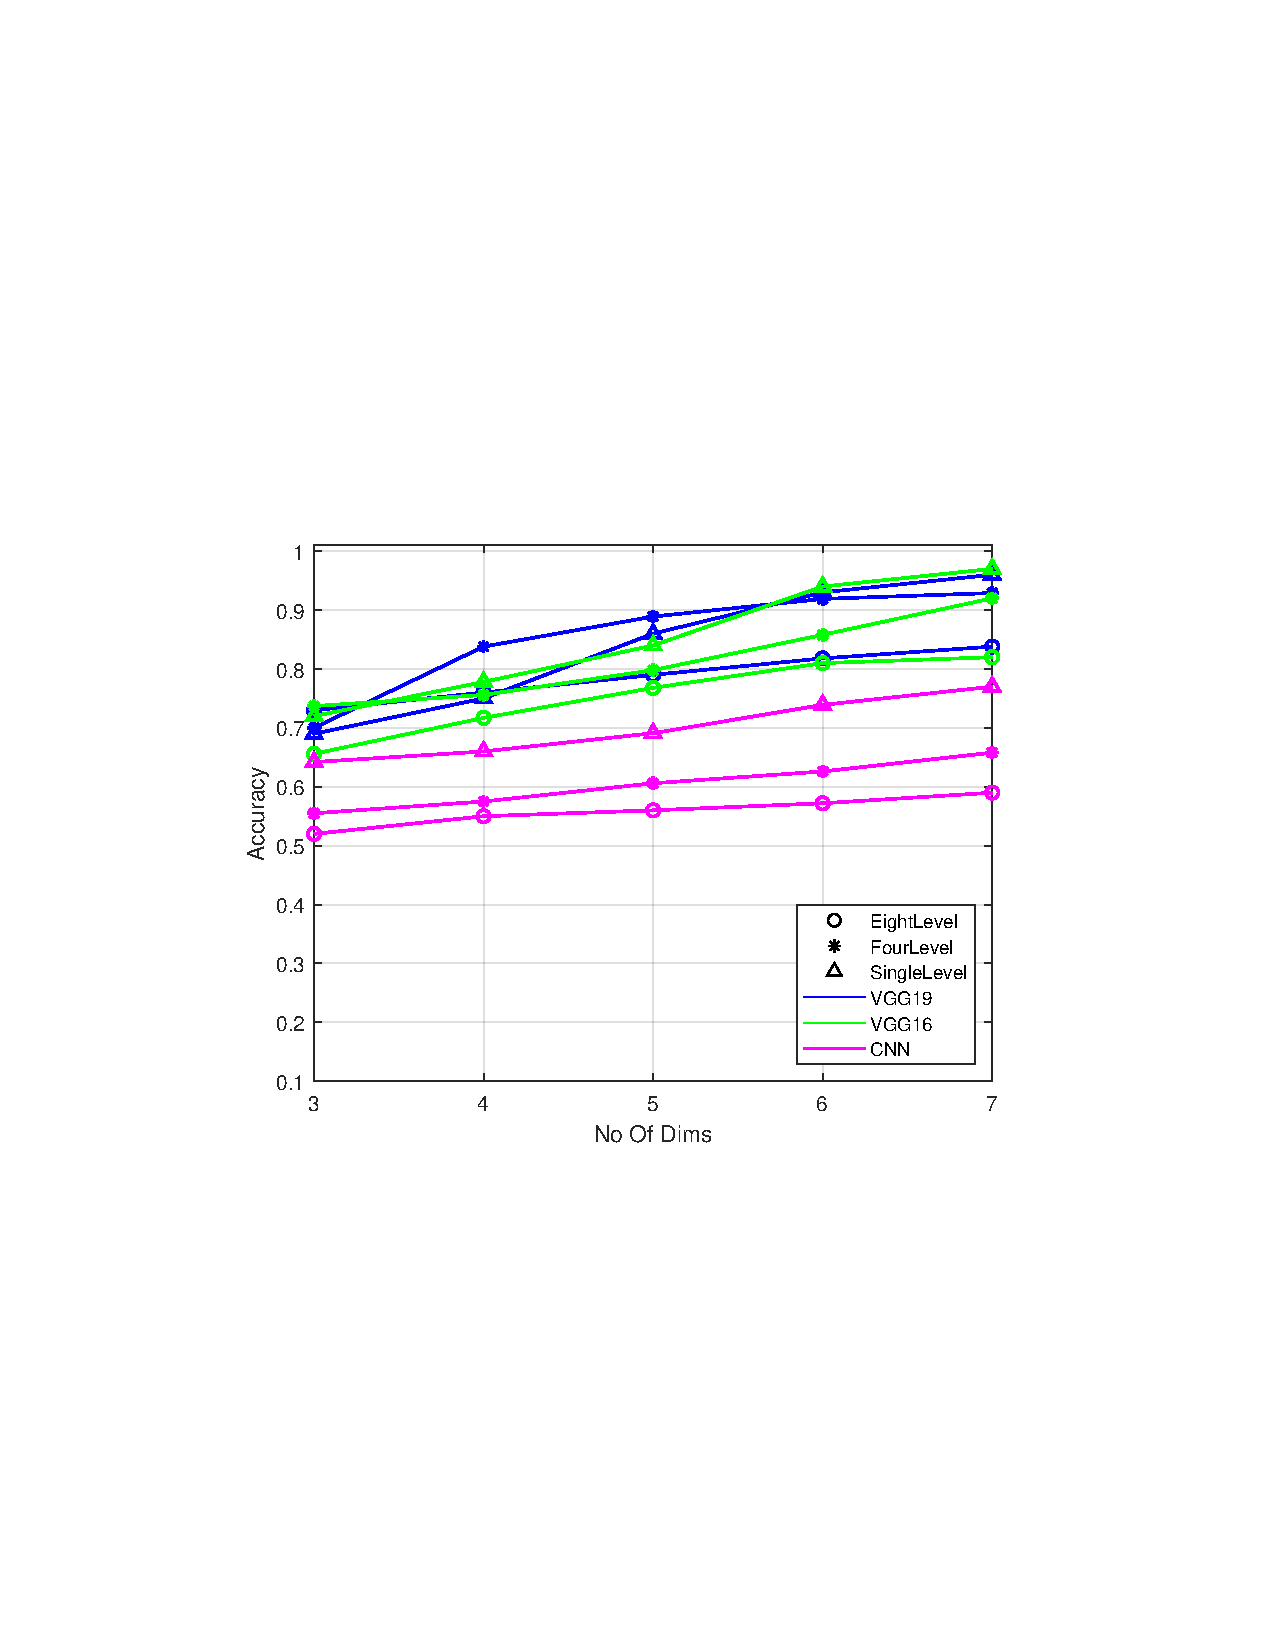
\includegraphics[width=\linewidth, trim=3.8cm 8cm 4cm 8cm, clip=true]{figures/att_acc}
		\captionsetup{justification=centering}
		\caption{ AT\&T}
		\label{fig:att_acc}
	\end{subfigure}
	\begin{subfigure}{.33\textwidth}
		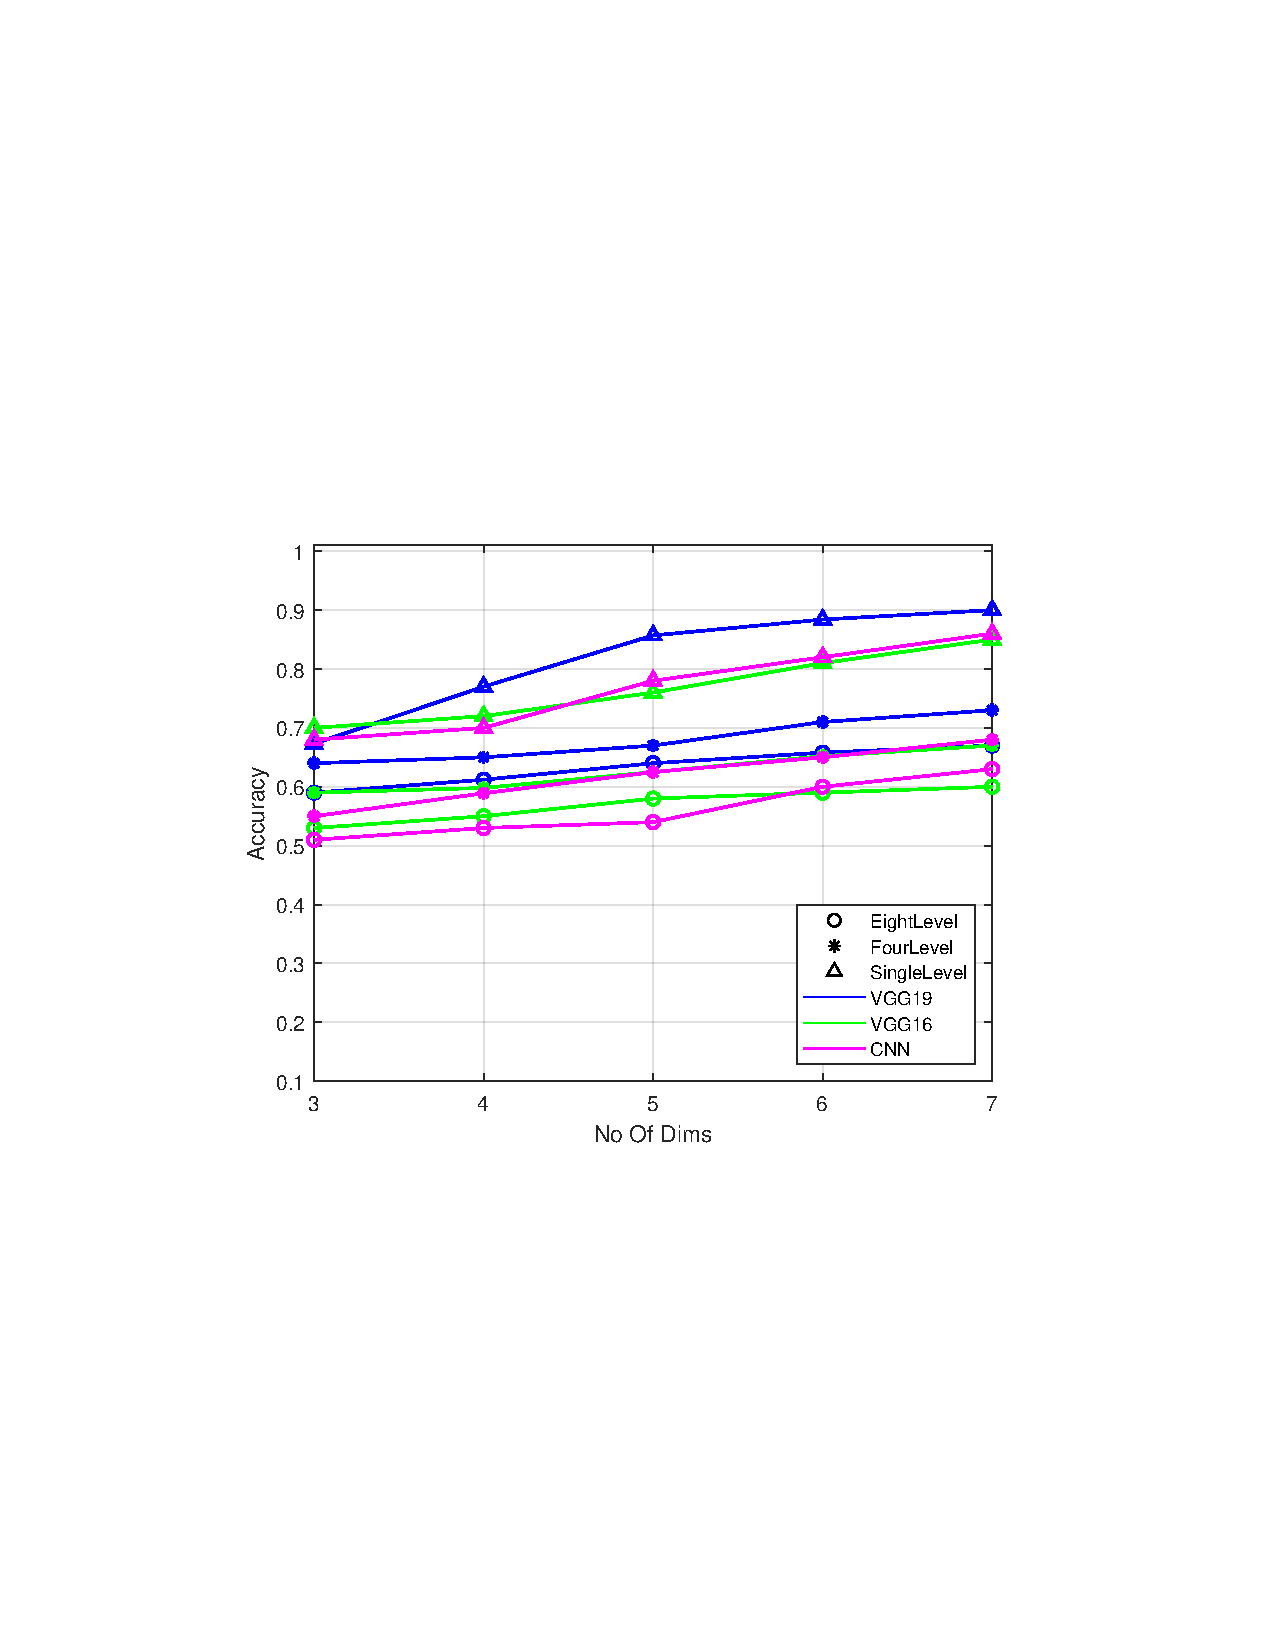
\includegraphics[width=\linewidth, trim=3.8cm 8cm 4cm 8cm, clip=true]{figures/yale_acc}
		\captionsetup{justification=centering}
		\caption{Yale\_B}
		\label{fig:yale_acc}
	\end{subfigure}
	\begin{subfigure}{.33\textwidth}
		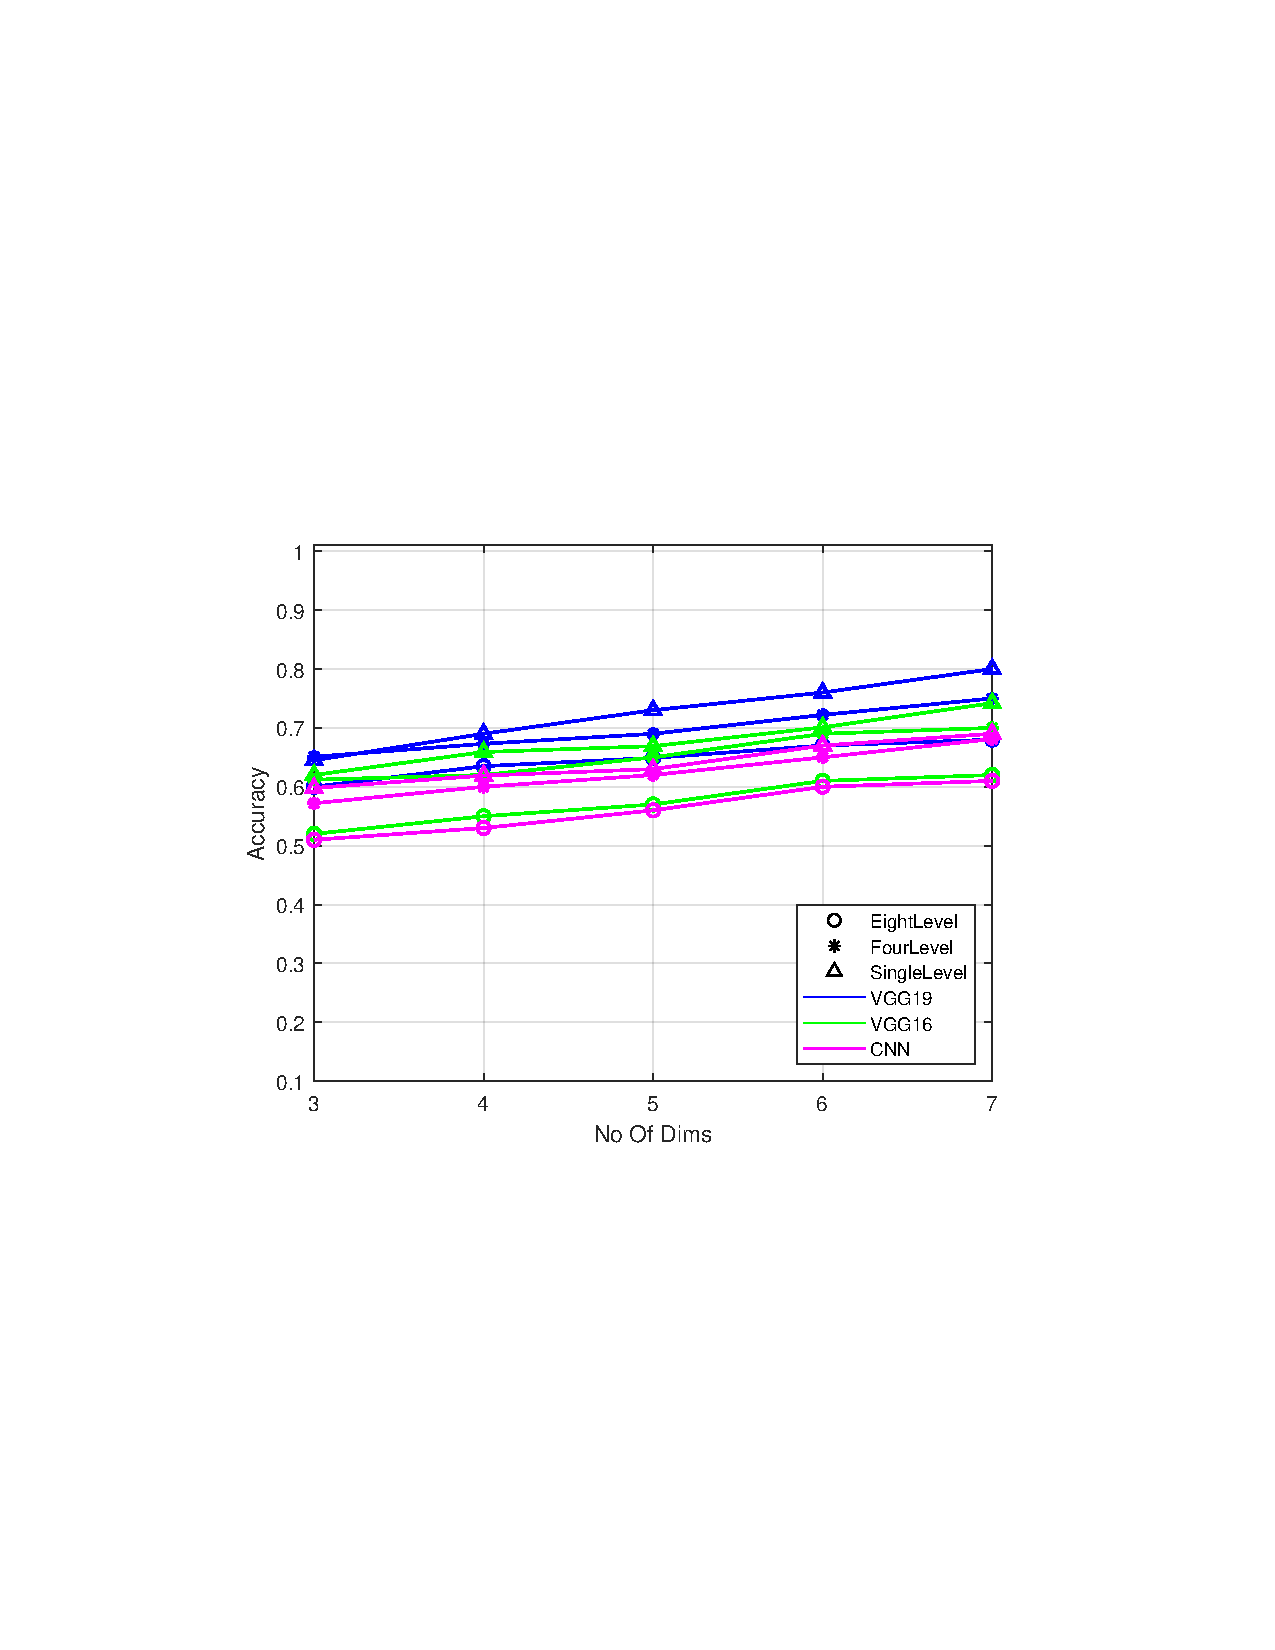
\includegraphics[width=\linewidth, trim=3.8cm 8cm 4cm 8cm, clip=true]{figures/celeba_acc}
		\captionsetup{justification=centering}
		\caption{CelebA}
		\label{fig:celeba_acc}
	\end{subfigure}
	\caption{Accuracy for Different Number of Reduced Dimensions }
	\label{fig:acc}
\end{figure*}

\begin{figure*}[ht!]
	\begin{subfigure}{.33\textwidth}
		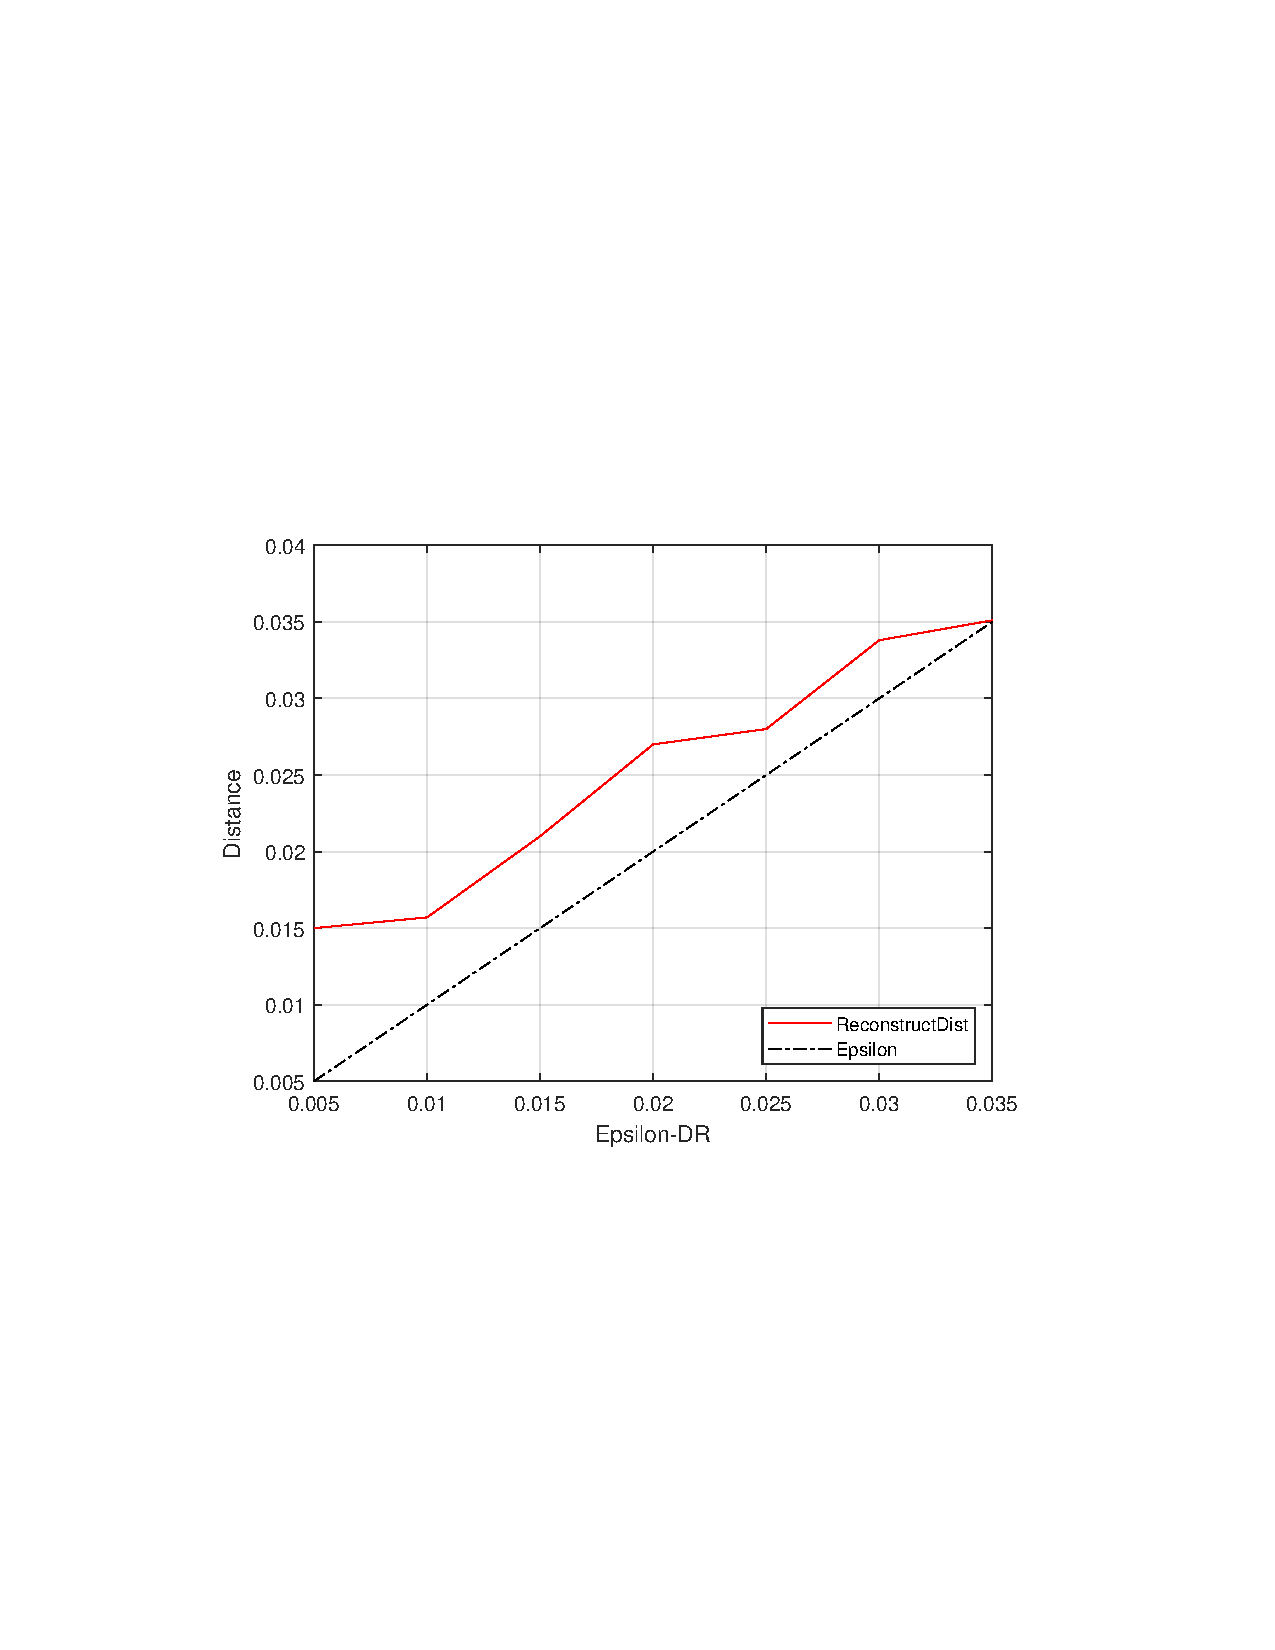
\includegraphics[width=\linewidth, trim=3.8cm 8cm 4cm 8cm, clip=true]{figures/ep_att}
		\captionsetup{justification=centering}
		\caption{ AT\&T}
		\label{fig:att_dist}
	\end{subfigure}
	\begin{subfigure}{.33\textwidth}
		\includegraphics[width=\linewidth, trim=3.8cm 8cm 4cm 8cm, clip=true]{figures/ep_yale}
		\captionsetup{justification=centering}
		\caption{Yale\_B}
		\label{fig:yale_dist}
	\end{subfigure}
	\begin{subfigure}{.33\textwidth}
		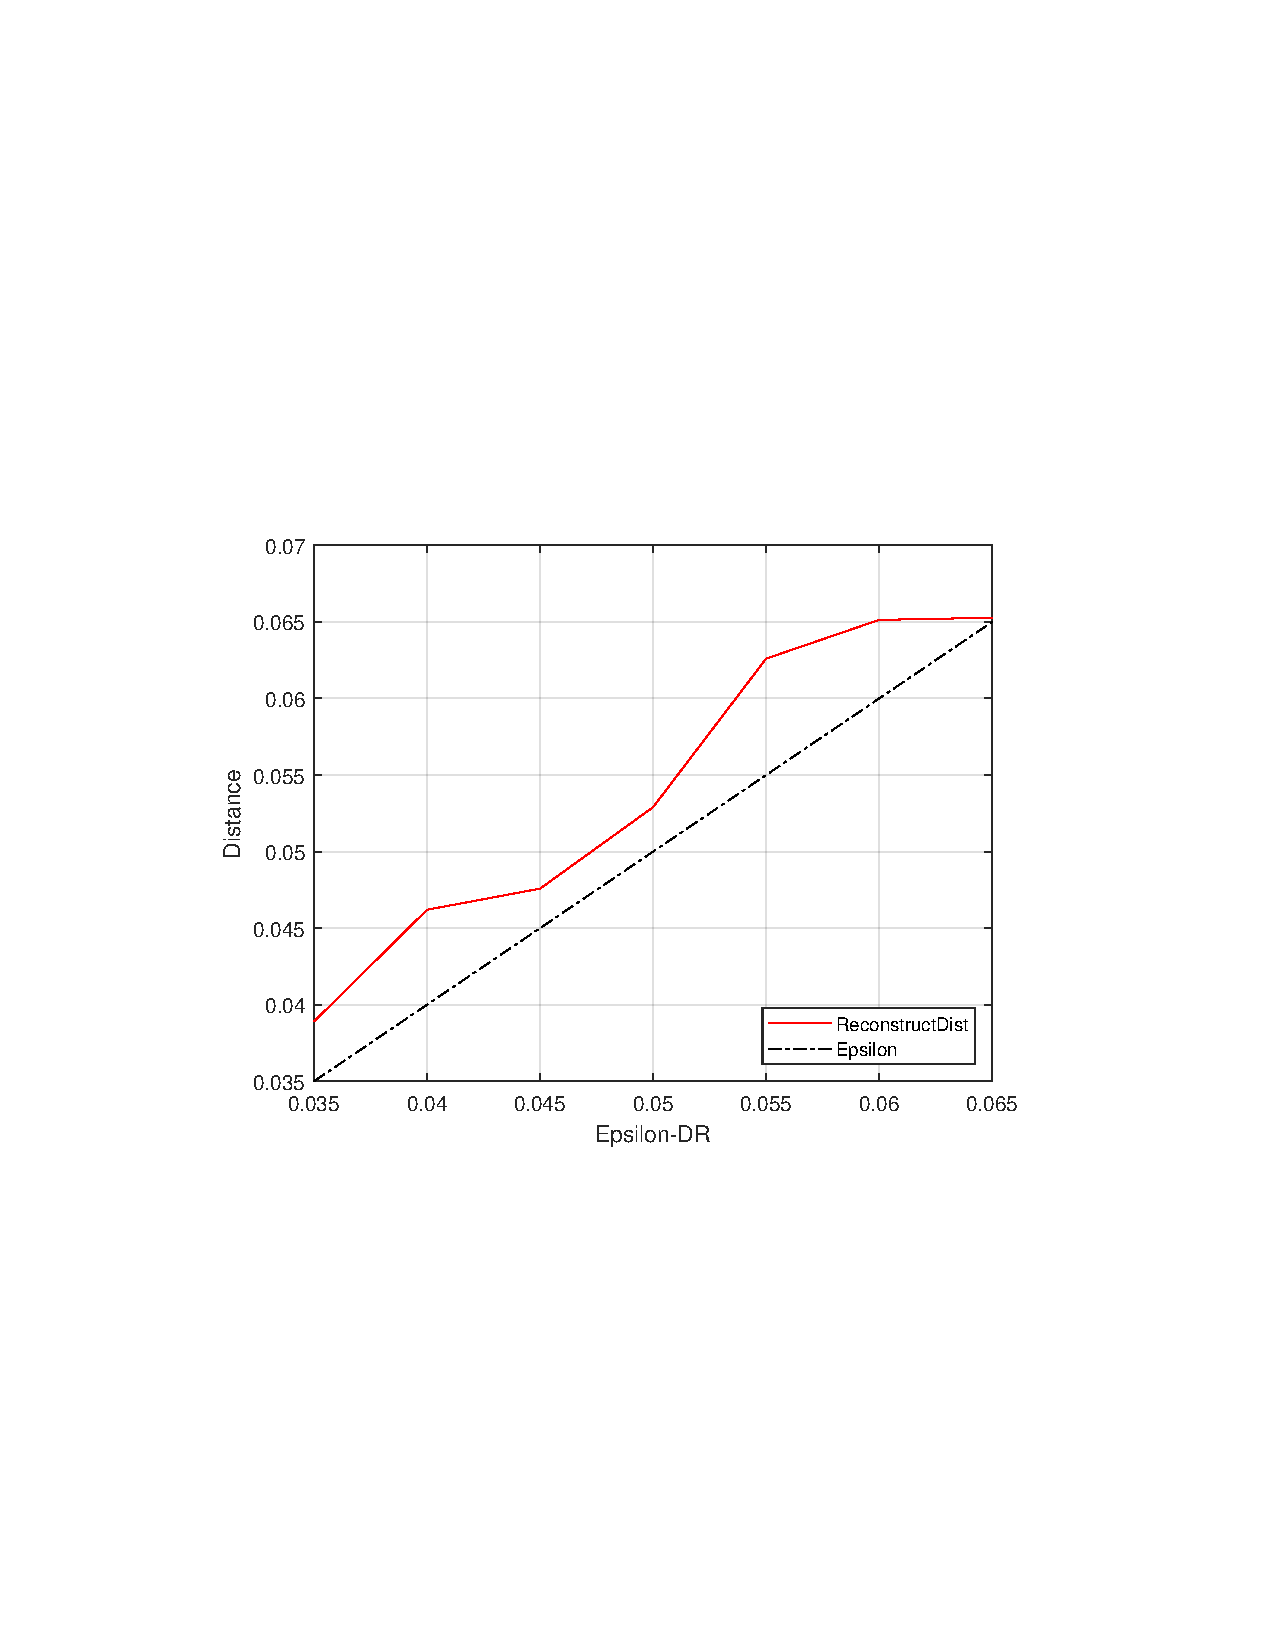
\includegraphics[width=\linewidth, trim=3.8cm 8cm 4cm 8cm, clip=true]{figures/ep_celeba}
		\captionsetup{justification=centering}
		\caption{CelebA}
		\label{fig:celeba_dist}
	\end{subfigure}
	\caption{Average Distance Measurement Result \{ 7 dimensions, Single-Level\}}
	\label{fig:distresult}
\end{figure*}
"


\setcounter{section}{5} "
\section{Visual Comparison to Privacy Preserving Techniques }
\label{AutoGAN_DP_PCA}

In this section, we compare AutoGAN-DRP with other privacy preserving methods in terms of ability to visually identify client's identities. We choose the widely used tool for privacy preserving Differential Privacy (DP) [27] and another privacy preservation method utilizing dimensionality reduction technique (i.e., Principle Component Analysis [34] ).

In these experiments, we implement AutoGAN-DRP following VGG19 structure for the Generator and Re-constructor, and other setting parameters (e.g., number of hidden layers, learning rate, optimization) are shown in Table \ref{table:implementation}. The images are reduced to seven dimensions for different values of $\epsilon$-DR to achieve different distances and accuracies. The datasets are grouped into two groups corresponding to a binary classifier. 

For implementing DP, we first generate a classifier on the authentication server by training the datasets with a VGG19 binary classifier (the structure of hidden layers is similar to our Generator in Table \ref{table:implementation}). The testing images are then perturbed using differential privacy method. Specifically, Laplace noise is added to the images with the sensitivity coefficient of 1 (it is computed by the maximum range value of each pixel [0,1]) and different DP epsilon parameters (this DP epsilon is different from our $\epsilon$-DR). The perturbed images are then sent to the authentication server and fed to the classifier. We visually compare the perturbed images of this method with AutoGAN. 

In addition, we follow instruction in FRiPAL [11] in which the clients reduce image dimension using Principle Component Analysis (PCA) and send reduced features to the server. FRiPAL claims that by reducing image dimension, their method can be more resilient to reconstruction attacks. The experiments are conducted with different number of reduced dimension. The images are reconstructed using \textit{Moore–Penrose inverse} method with assumption that an adversary has assess to the model. The classification accuracy is evaluated using a classifier which has similar structure to AutoGAN's classifier. 

Table \ref{table:visualization} shows image samples and results over the three datasets. Overall, AutoGAN-DRP is more resilient to reconstruction attacks compared to the other two techniques. For instance, at the accuracy of 79\% on AT\&T dataset, 80\% on YaleB, and 73\% on CelebA, we cannot distinguish entities from the others. For DP method, the accuracy decreases when the DP epsilon decreases (adding more noise), and the perturbed images become harder to recognize. However, at a low accuracy 57\%, we are still able to distinguish identities by human eyes. The reason is that DP noise does not focus on the important visual pixels. For PCA, the accuracy also goes down when the number of dimensions decreases and the distances increase. Since PCA transformation is linear and deterministic, the original information can be significantly reconstructed using the inverse transformation deriving from the model or training data. Thus, at the accuracy of 75\% on AT\&T, 71\% on YaleB, and 68\% on CelebA, we still can differentiate individuals. Overall, our proposed method shows the advantage in securing the data while retaining high data utility.       
\\ 
\setcounter{table}{1}

\begin{table}[H]
	\centering
	%trim  left, bottom, right and top 
	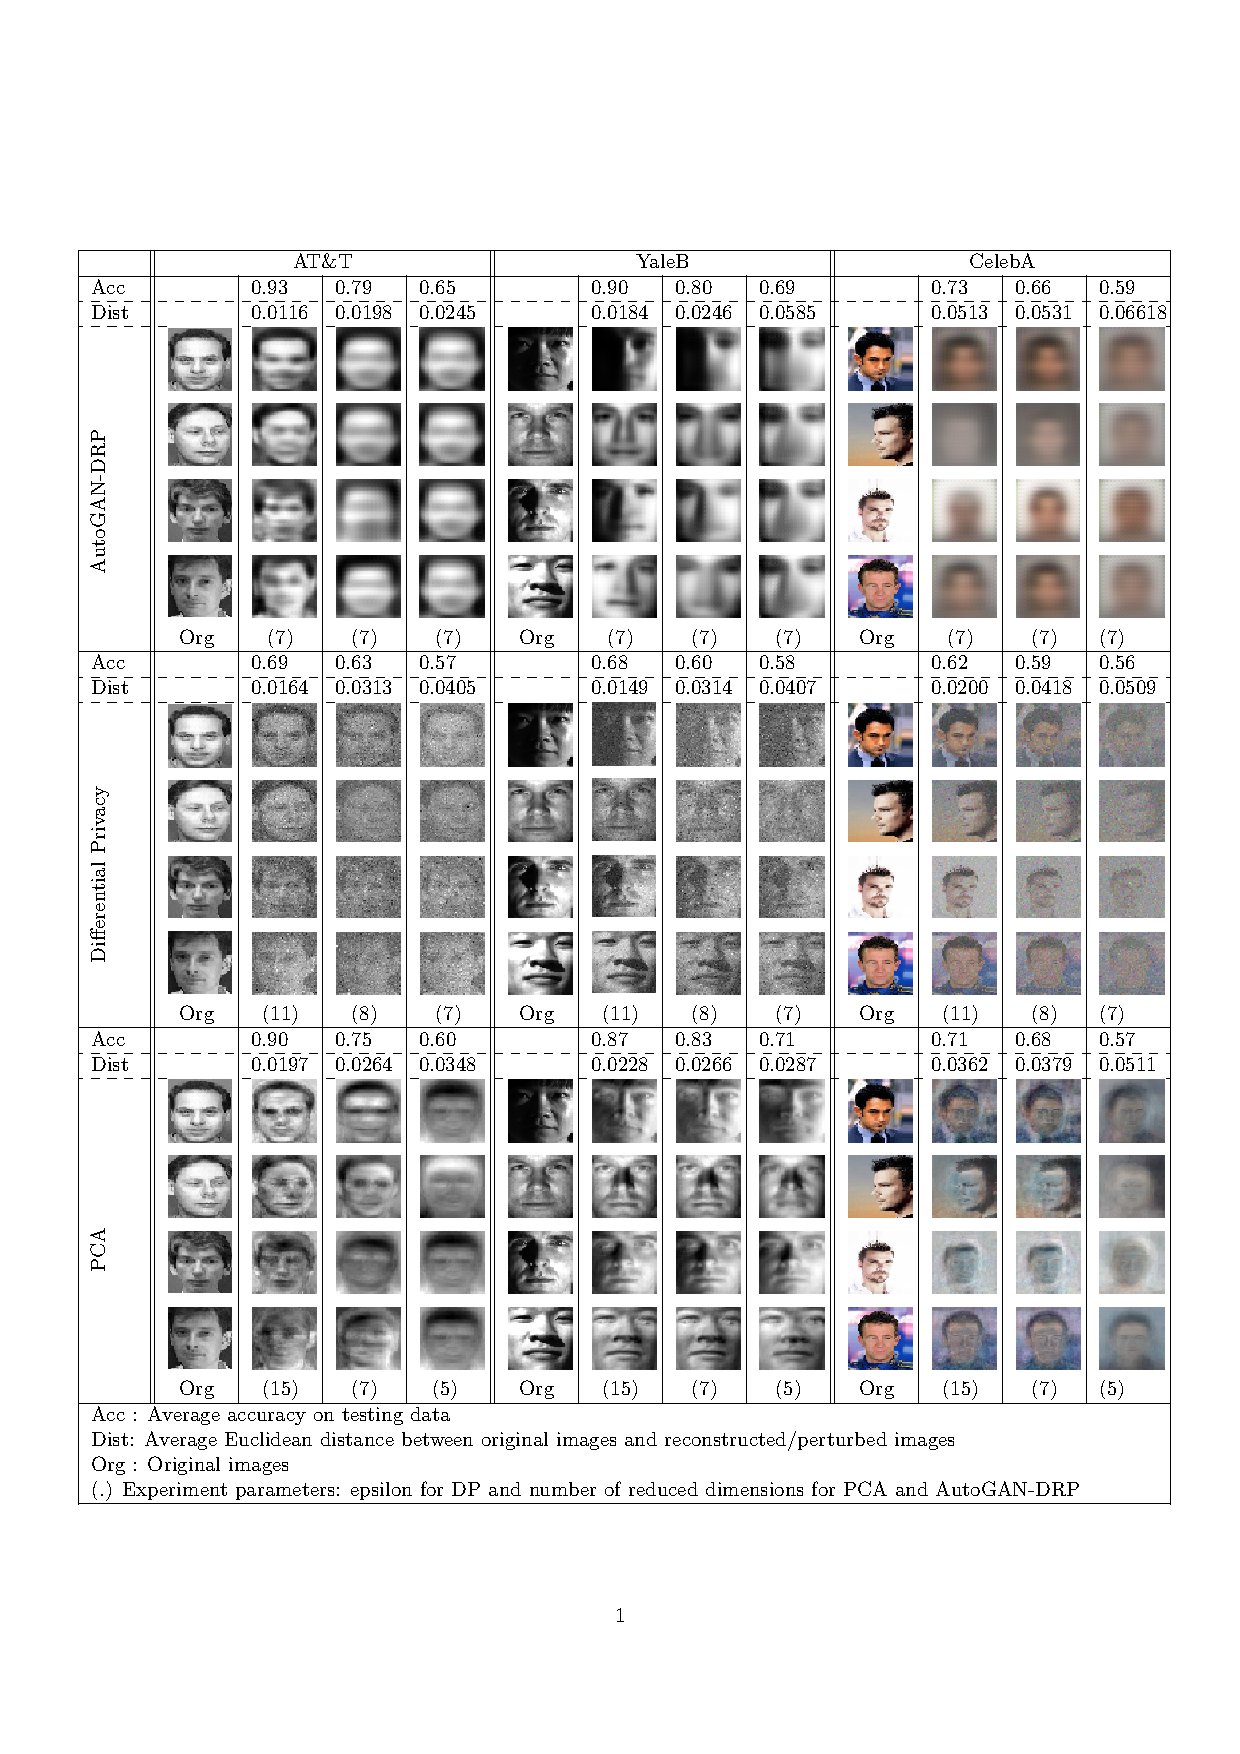
\includegraphics[width=0.8\linewidth, trim=1cm 3cm 1cm 3cm, clip=true]{tables/img_table}
	\caption{Sample visualization of AutoGAN, DP, PCA over three datasets}
	\label{table:visualization}
\end{table}

"